% Options for packages loaded elsewhere
\PassOptionsToPackage{unicode}{hyperref}
\PassOptionsToPackage{hyphens}{url}
\PassOptionsToPackage{dvipsnames,svgnames*,x11names*}{xcolor}
%
\documentclass[
  10pt,
]{article}
\usepackage{amsmath,amssymb}
\usepackage{lmodern}
\usepackage{ifxetex,ifluatex}
\ifnum 0\ifxetex 1\fi\ifluatex 1\fi=0 % if pdftex
  \usepackage[T1]{fontenc}
  \usepackage[utf8]{inputenc}
  \usepackage{textcomp} % provide euro and other symbols
\else % if luatex or xetex
  \usepackage{unicode-math}
  \defaultfontfeatures{Scale=MatchLowercase}
  \defaultfontfeatures[\rmfamily]{Ligatures=TeX,Scale=1}
\fi
% Use upquote if available, for straight quotes in verbatim environments
\IfFileExists{upquote.sty}{\usepackage{upquote}}{}
\IfFileExists{microtype.sty}{% use microtype if available
  \usepackage[]{microtype}
  \UseMicrotypeSet[protrusion]{basicmath} % disable protrusion for tt fonts
}{}
\makeatletter
\@ifundefined{KOMAClassName}{% if non-KOMA class
  \IfFileExists{parskip.sty}{%
    \usepackage{parskip}
  }{% else
    \setlength{\parindent}{0pt}
    \setlength{\parskip}{6pt plus 2pt minus 1pt}}
}{% if KOMA class
  \KOMAoptions{parskip=half}}
\makeatother
\usepackage{xcolor}
\IfFileExists{xurl.sty}{\usepackage{xurl}}{} % add URL line breaks if available
\IfFileExists{bookmark.sty}{\usepackage{bookmark}}{\usepackage{hyperref}}
\hypersetup{
  pdftitle={Construct and describe share data},
  pdfauthor={Suguru Otani},
  colorlinks=true,
  linkcolor=blue,
  filecolor=Maroon,
  citecolor=Blue,
  urlcolor=blue,
  pdfcreator={LaTeX via pandoc}}
\urlstyle{same} % disable monospaced font for URLs
\usepackage[margin=1in]{geometry}
\usepackage{graphicx}
\makeatletter
\def\maxwidth{\ifdim\Gin@nat@width>\linewidth\linewidth\else\Gin@nat@width\fi}
\def\maxheight{\ifdim\Gin@nat@height>\textheight\textheight\else\Gin@nat@height\fi}
\makeatother
% Scale images if necessary, so that they will not overflow the page
% margins by default, and it is still possible to overwrite the defaults
% using explicit options in \includegraphics[width, height, ...]{}
\setkeys{Gin}{width=\maxwidth,height=\maxheight,keepaspectratio}
% Set default figure placement to htbp
\makeatletter
\def\fps@figure{htbp}
\makeatother
\setlength{\emergencystretch}{3em} % prevent overfull lines
\providecommand{\tightlist}{%
  \setlength{\itemsep}{0pt}\setlength{\parskip}{0pt}}
\setcounter{secnumdepth}{5}
\usepackage{float}
\usepackage{booktabs}
\usepackage{pdfpages}
\usepackage{threeparttable}
\usepackage[labelfont=bf]{caption}
\usepackage{bookmark}
\ifluatex
  \usepackage{selnolig}  % disable illegal ligatures
\fi

\title{Construct and describe share data}
\author{Suguru Otani\footnote{\href{mailto:so19@rice.edu}{\nolinkurl{so19@rice.edu}},
  Rice University}}
\date{Oct 22 2020}

\begin{document}
\maketitle

\hypertarget{overview}{%
\section{Overview}\label{overview}}

This file generates the following figures and tables.

\begin{itemize}
\tightlist
\item
  Figures 2, 3, 4, 5, and 9.
\item
  Tables 2, 3, 4, and 5.
\end{itemize}

All raw data must be located in ../input folder. All outputs will be
located in ../figuretable folder or ../output folder.

Note that Table 1 does not contain the information about data and
Figures 6, 7, and 8 are generated in ship\_merger\_score\_estimation.jl.

\hypertarget{figures}{%
\section{Figures}\label{figures}}

\hypertarget{figure-1-the-trend-of-the-worlds-shipping-gross-tonnage-1000-tons.}{%
\subsection{(Figure 1) The trend of the world's shipping gross tonnage
(1000
tons).}\label{figure-1-the-trend-of-the-worlds-shipping-gross-tonnage-1000-tons.}}

\begin{figure}[!ht]
\begin{center}
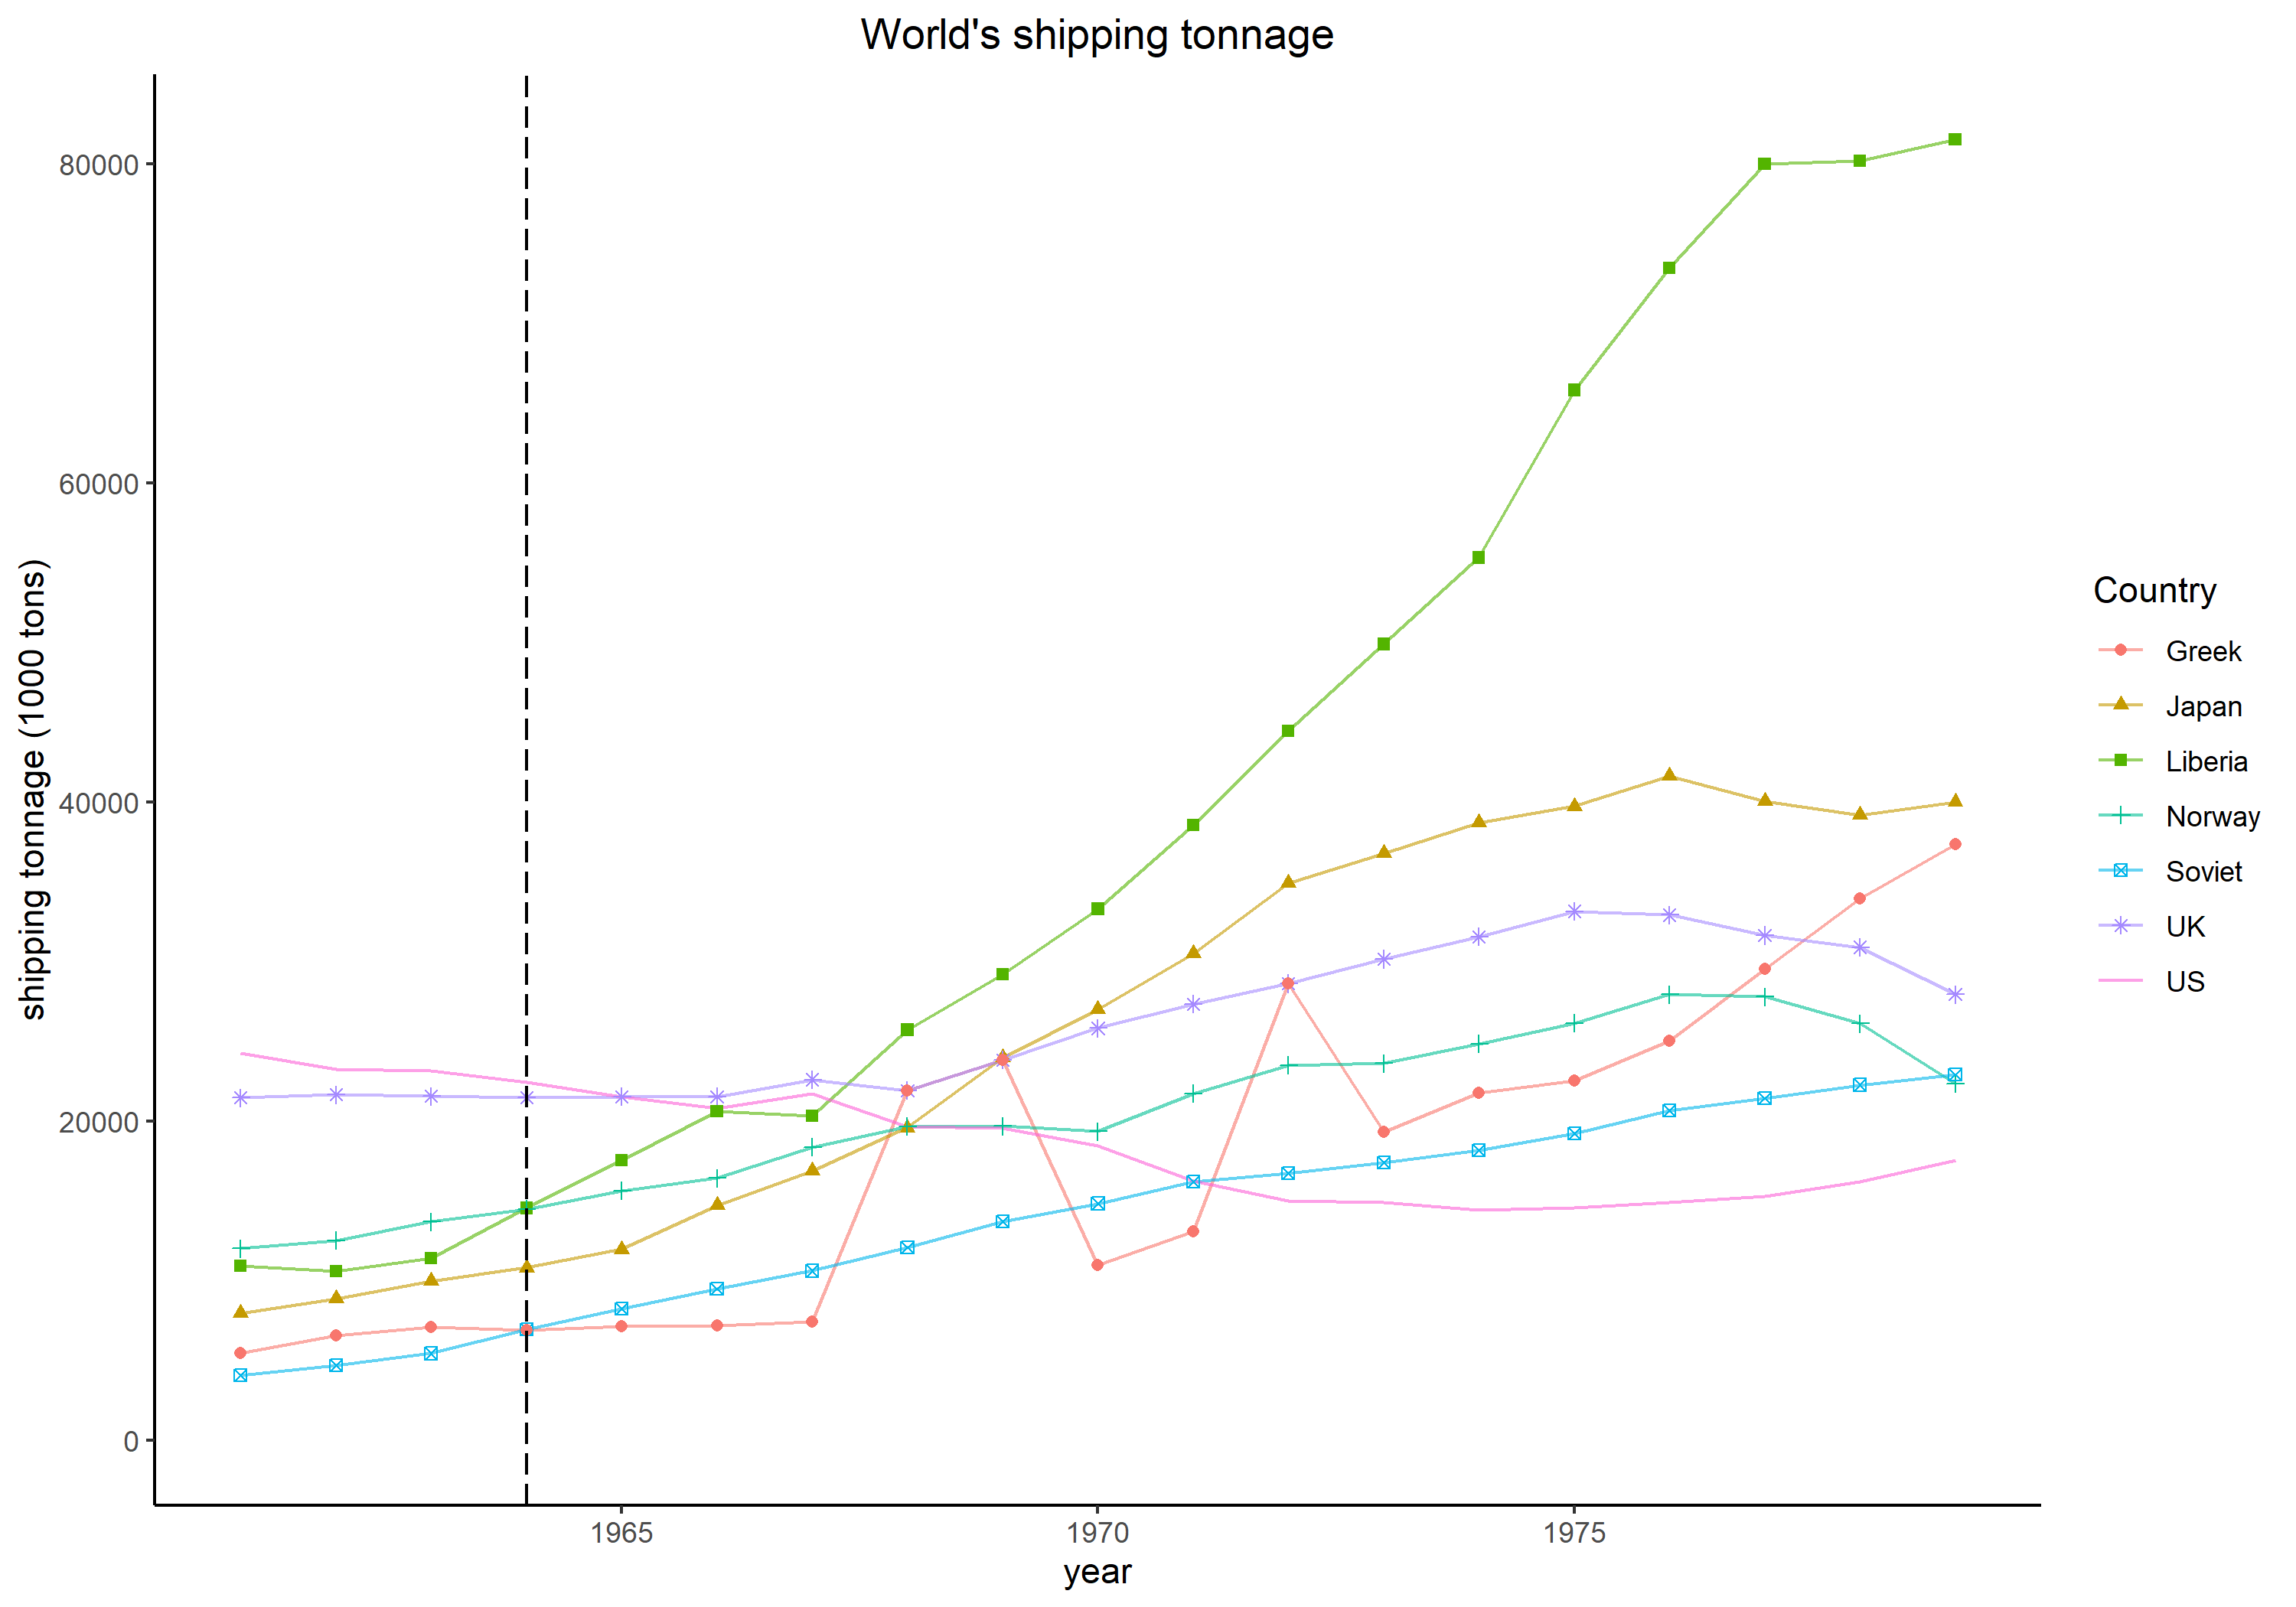
\includegraphics[height = 0.37\textheight]{../figuretable/shippingtonnage.png}
\end{center}
\caption{\textbf{The trend of world's shipping gross tonnage (1000 tons)}}
\label{fg:shippingtonnage}
\end{figure}

\hypertarget{load-main-data}{%
\section{Load main data}\label{load-main-data}}

\hypertarget{type-based-histogram}{%
\section{Type-based histogram}\label{type-based-histogram}}

\hypertarget{figure-2-configuration-of-tonnage-size-for-each-carrier-type}{%
\subsection{(Figure 2) Configuration of tonnage size for each carrier
type}\label{figure-2-configuration-of-tonnage-size-for-each-carrier-type}}

\begin{figure}[!ht]
\begin{center}
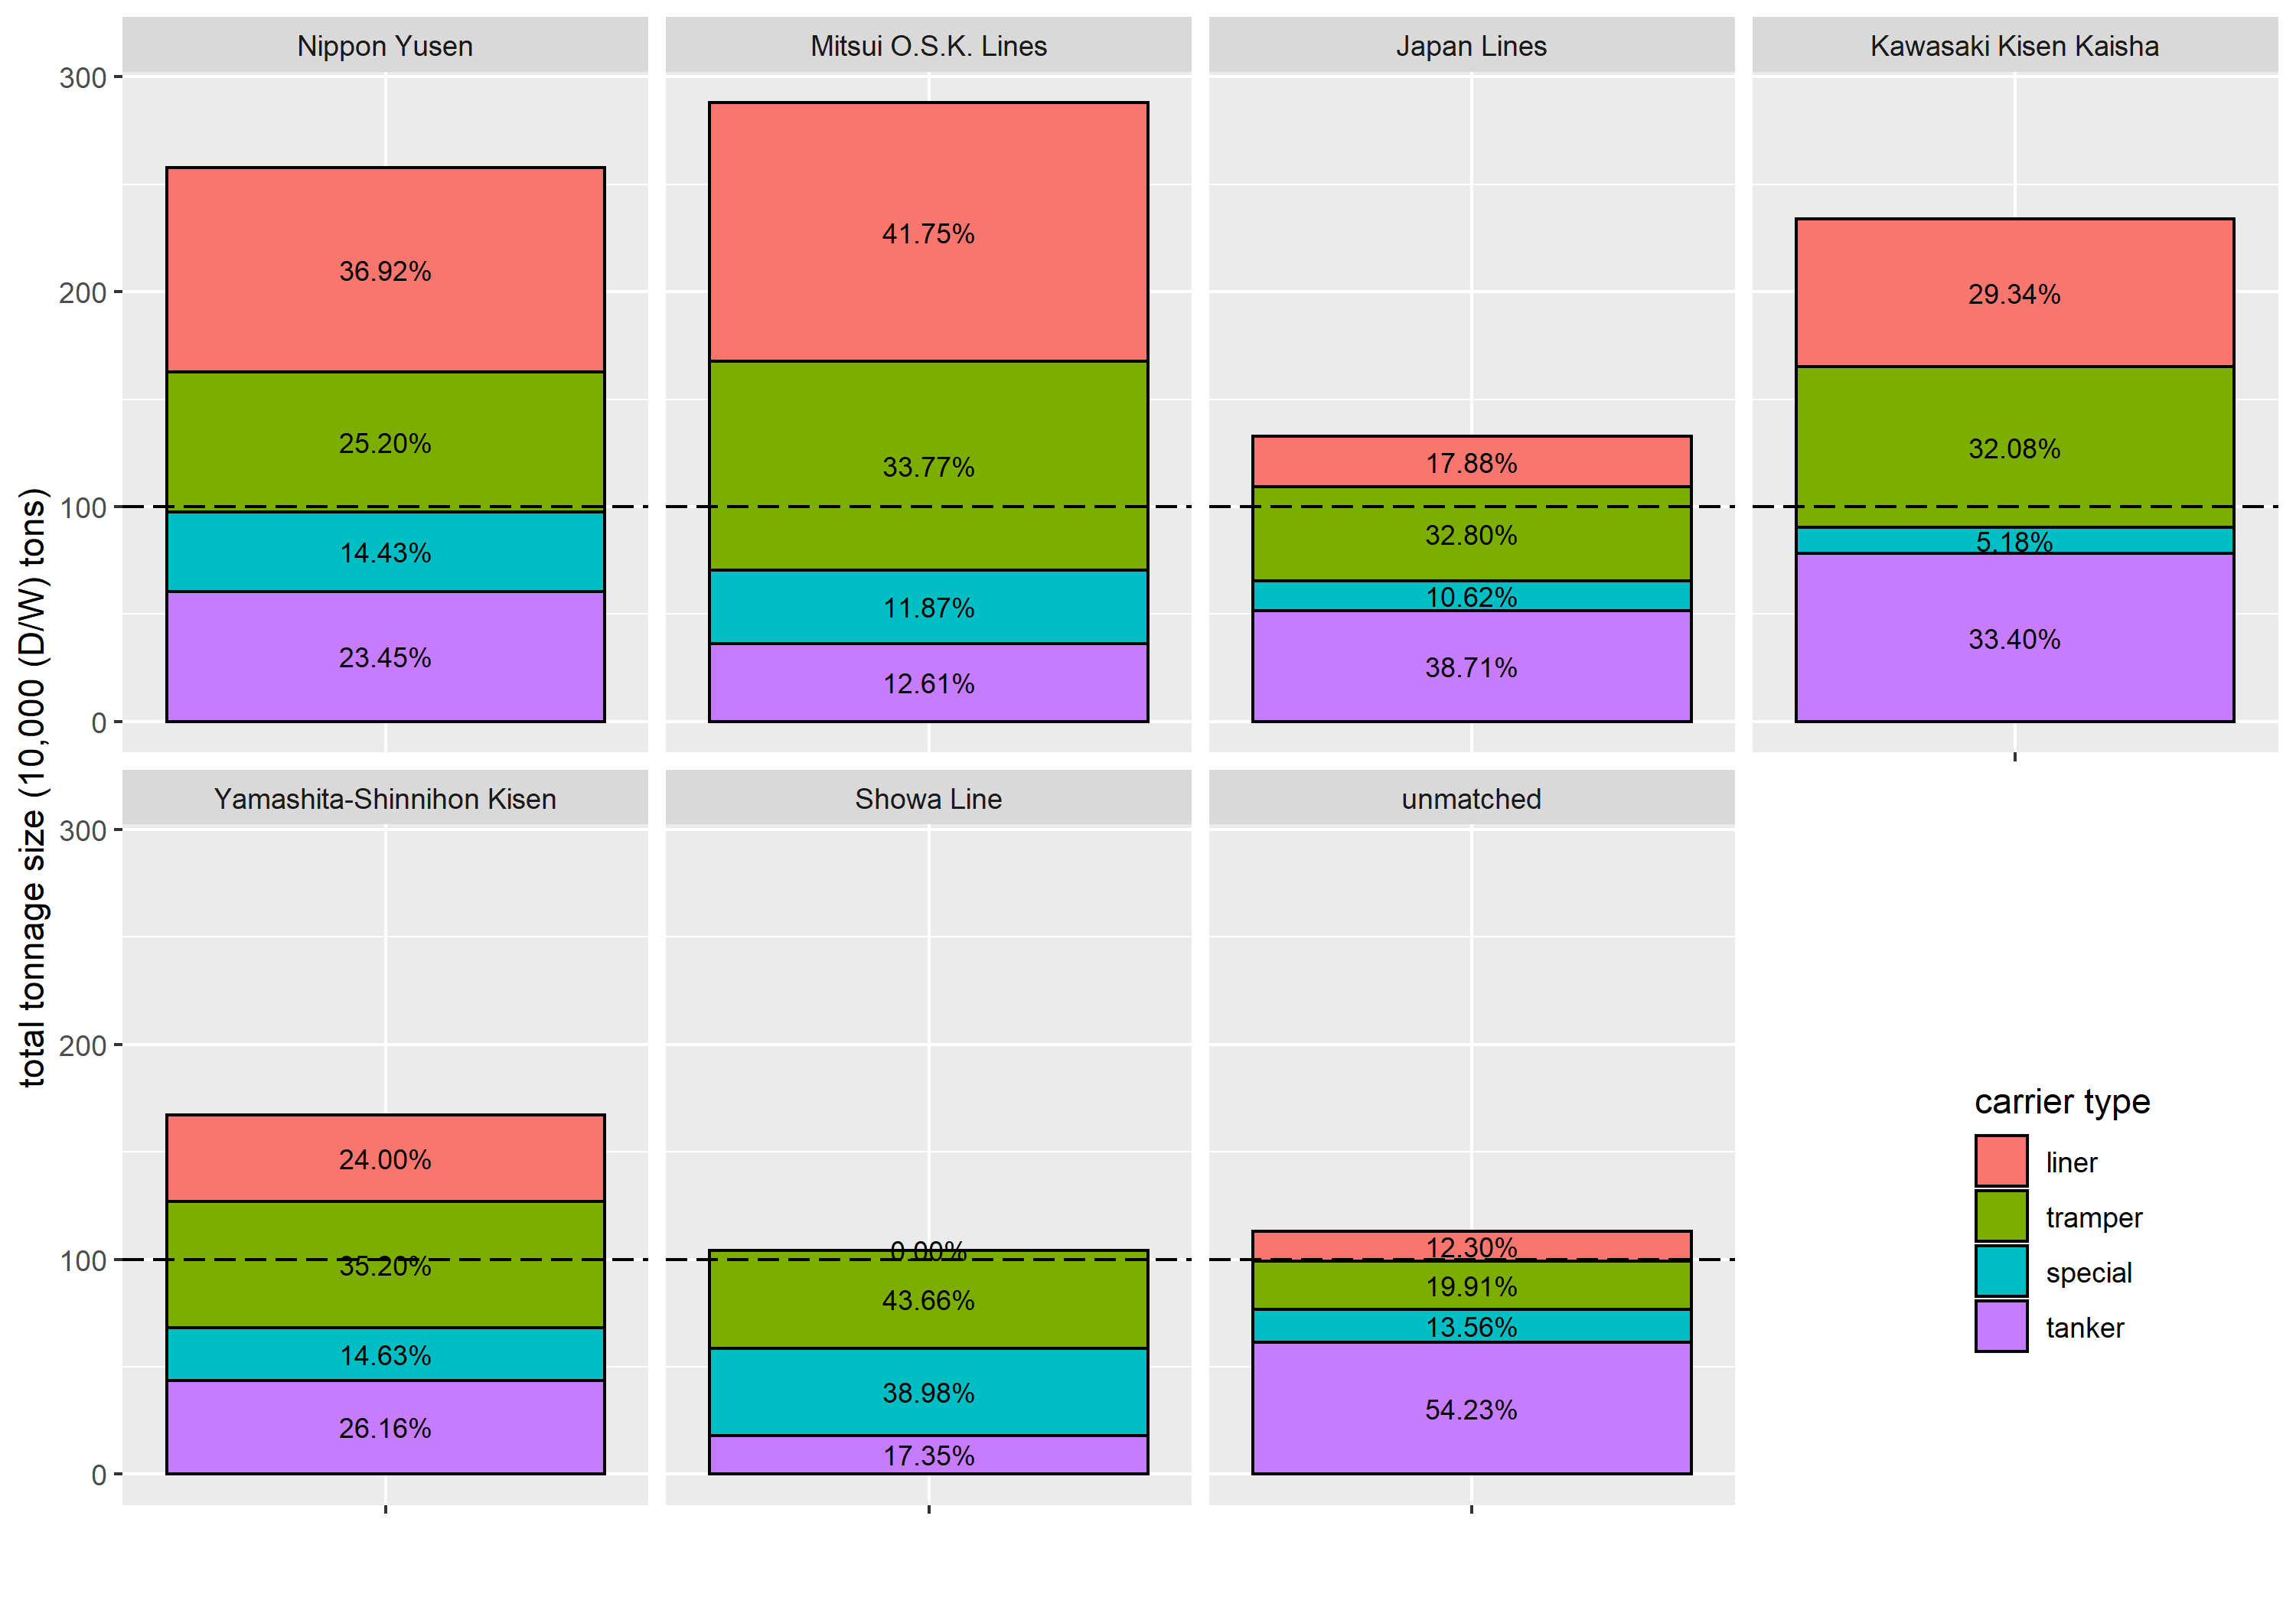
\includegraphics[height = 0.37\textheight]{../figuretable/carrier_composition_eachgroup.png}
\end{center}
\caption{\textbf{Configuration of tonnage size for each carrier type}. Observation unit: group-level total tonnage size for each carrier type after mergers. The dotted horizontal line indicates the subsidy threshold.}
\label{fg:carrier_composition_eachgroup}
\end{figure}

\hypertarget{figure-3-distribution-of-tonnage-size-for-each-firm-type.}{%
\subsection{(Figure 3) Distribution of tonnage size for each firm
type.}\label{figure-3-distribution-of-tonnage-size-for-each-firm-type.}}

\begin{figure}[!ht]
\begin{center}
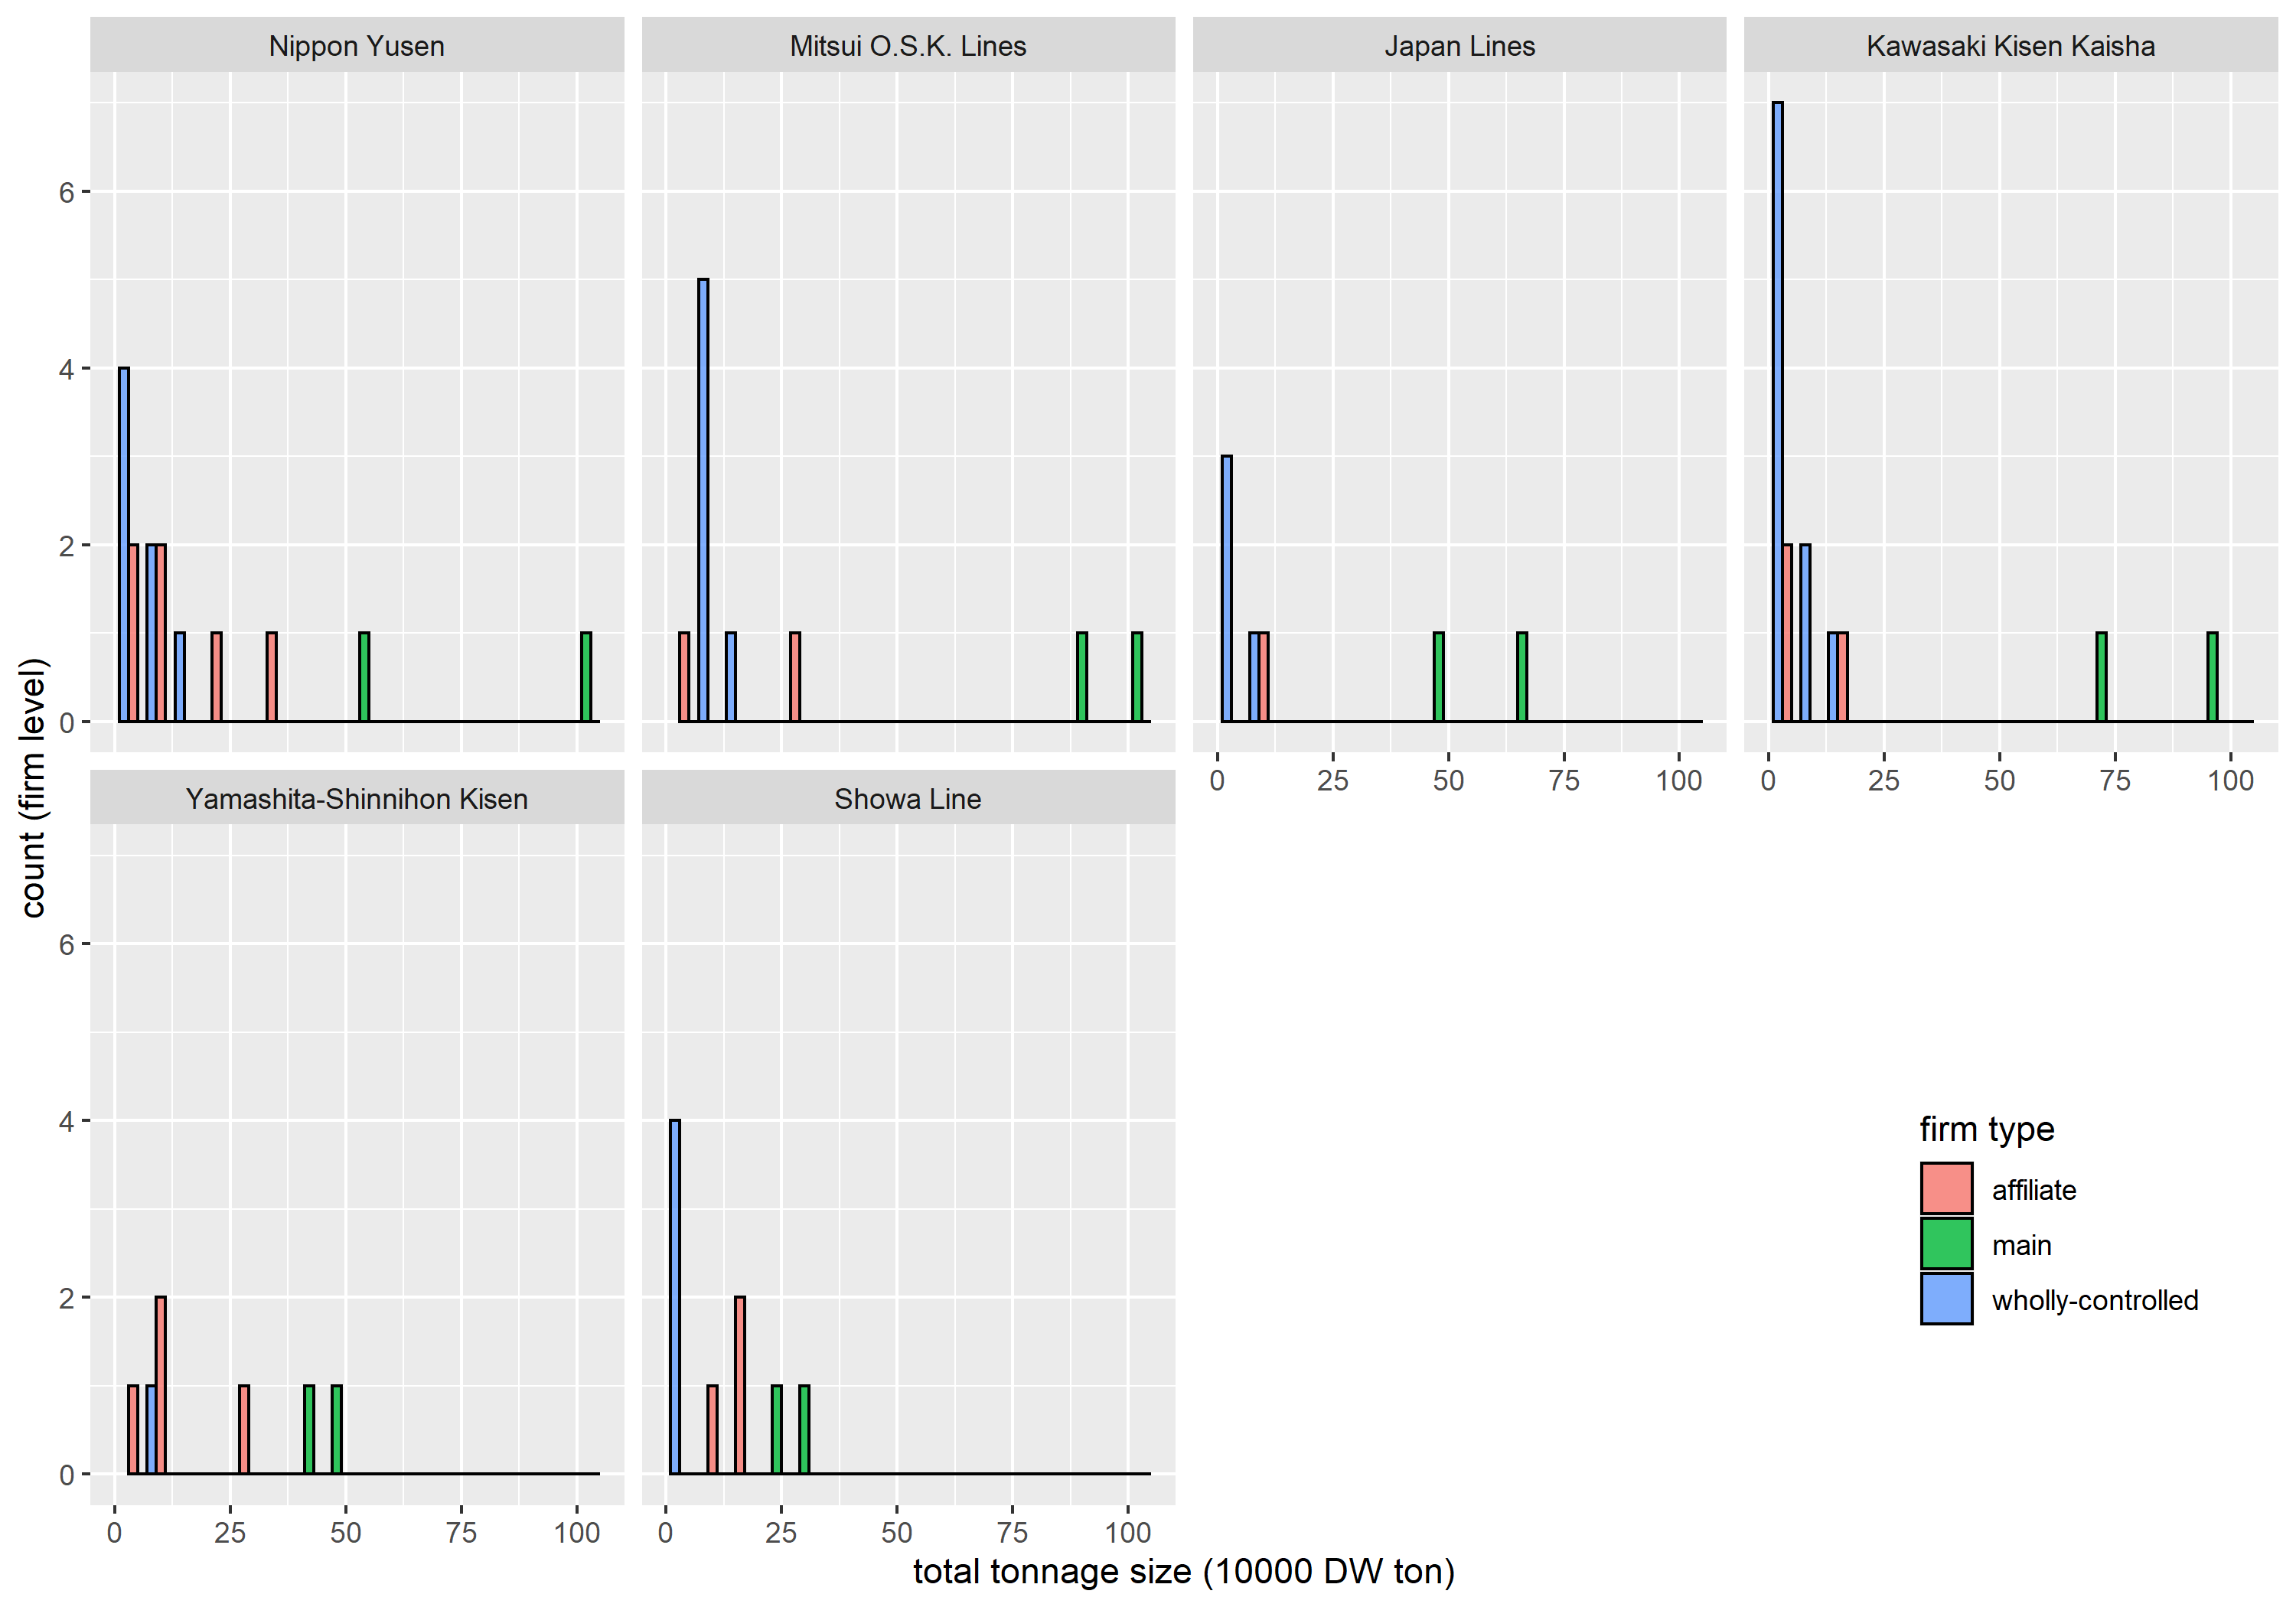
\includegraphics[height = 0.37\textheight]{../figuretable/type_dist_eachgroup.png}
\end{center}
\caption{\textbf{Distribution of tonnage size for each firm type}. Observation unit: the firm-level tonnage size for each firm type of each group after mergers.}
\label{fg:type_dist_eachgroup}
\end{figure}

\hypertarget{figure-4-distribution-of-tonnage-size-for-each-carrier-type.}{%
\subsection{(Figure 4) Distribution of tonnage size for each carrier
type.}\label{figure-4-distribution-of-tonnage-size-for-each-carrier-type.}}

\begin{figure}[!ht]
\begin{center}
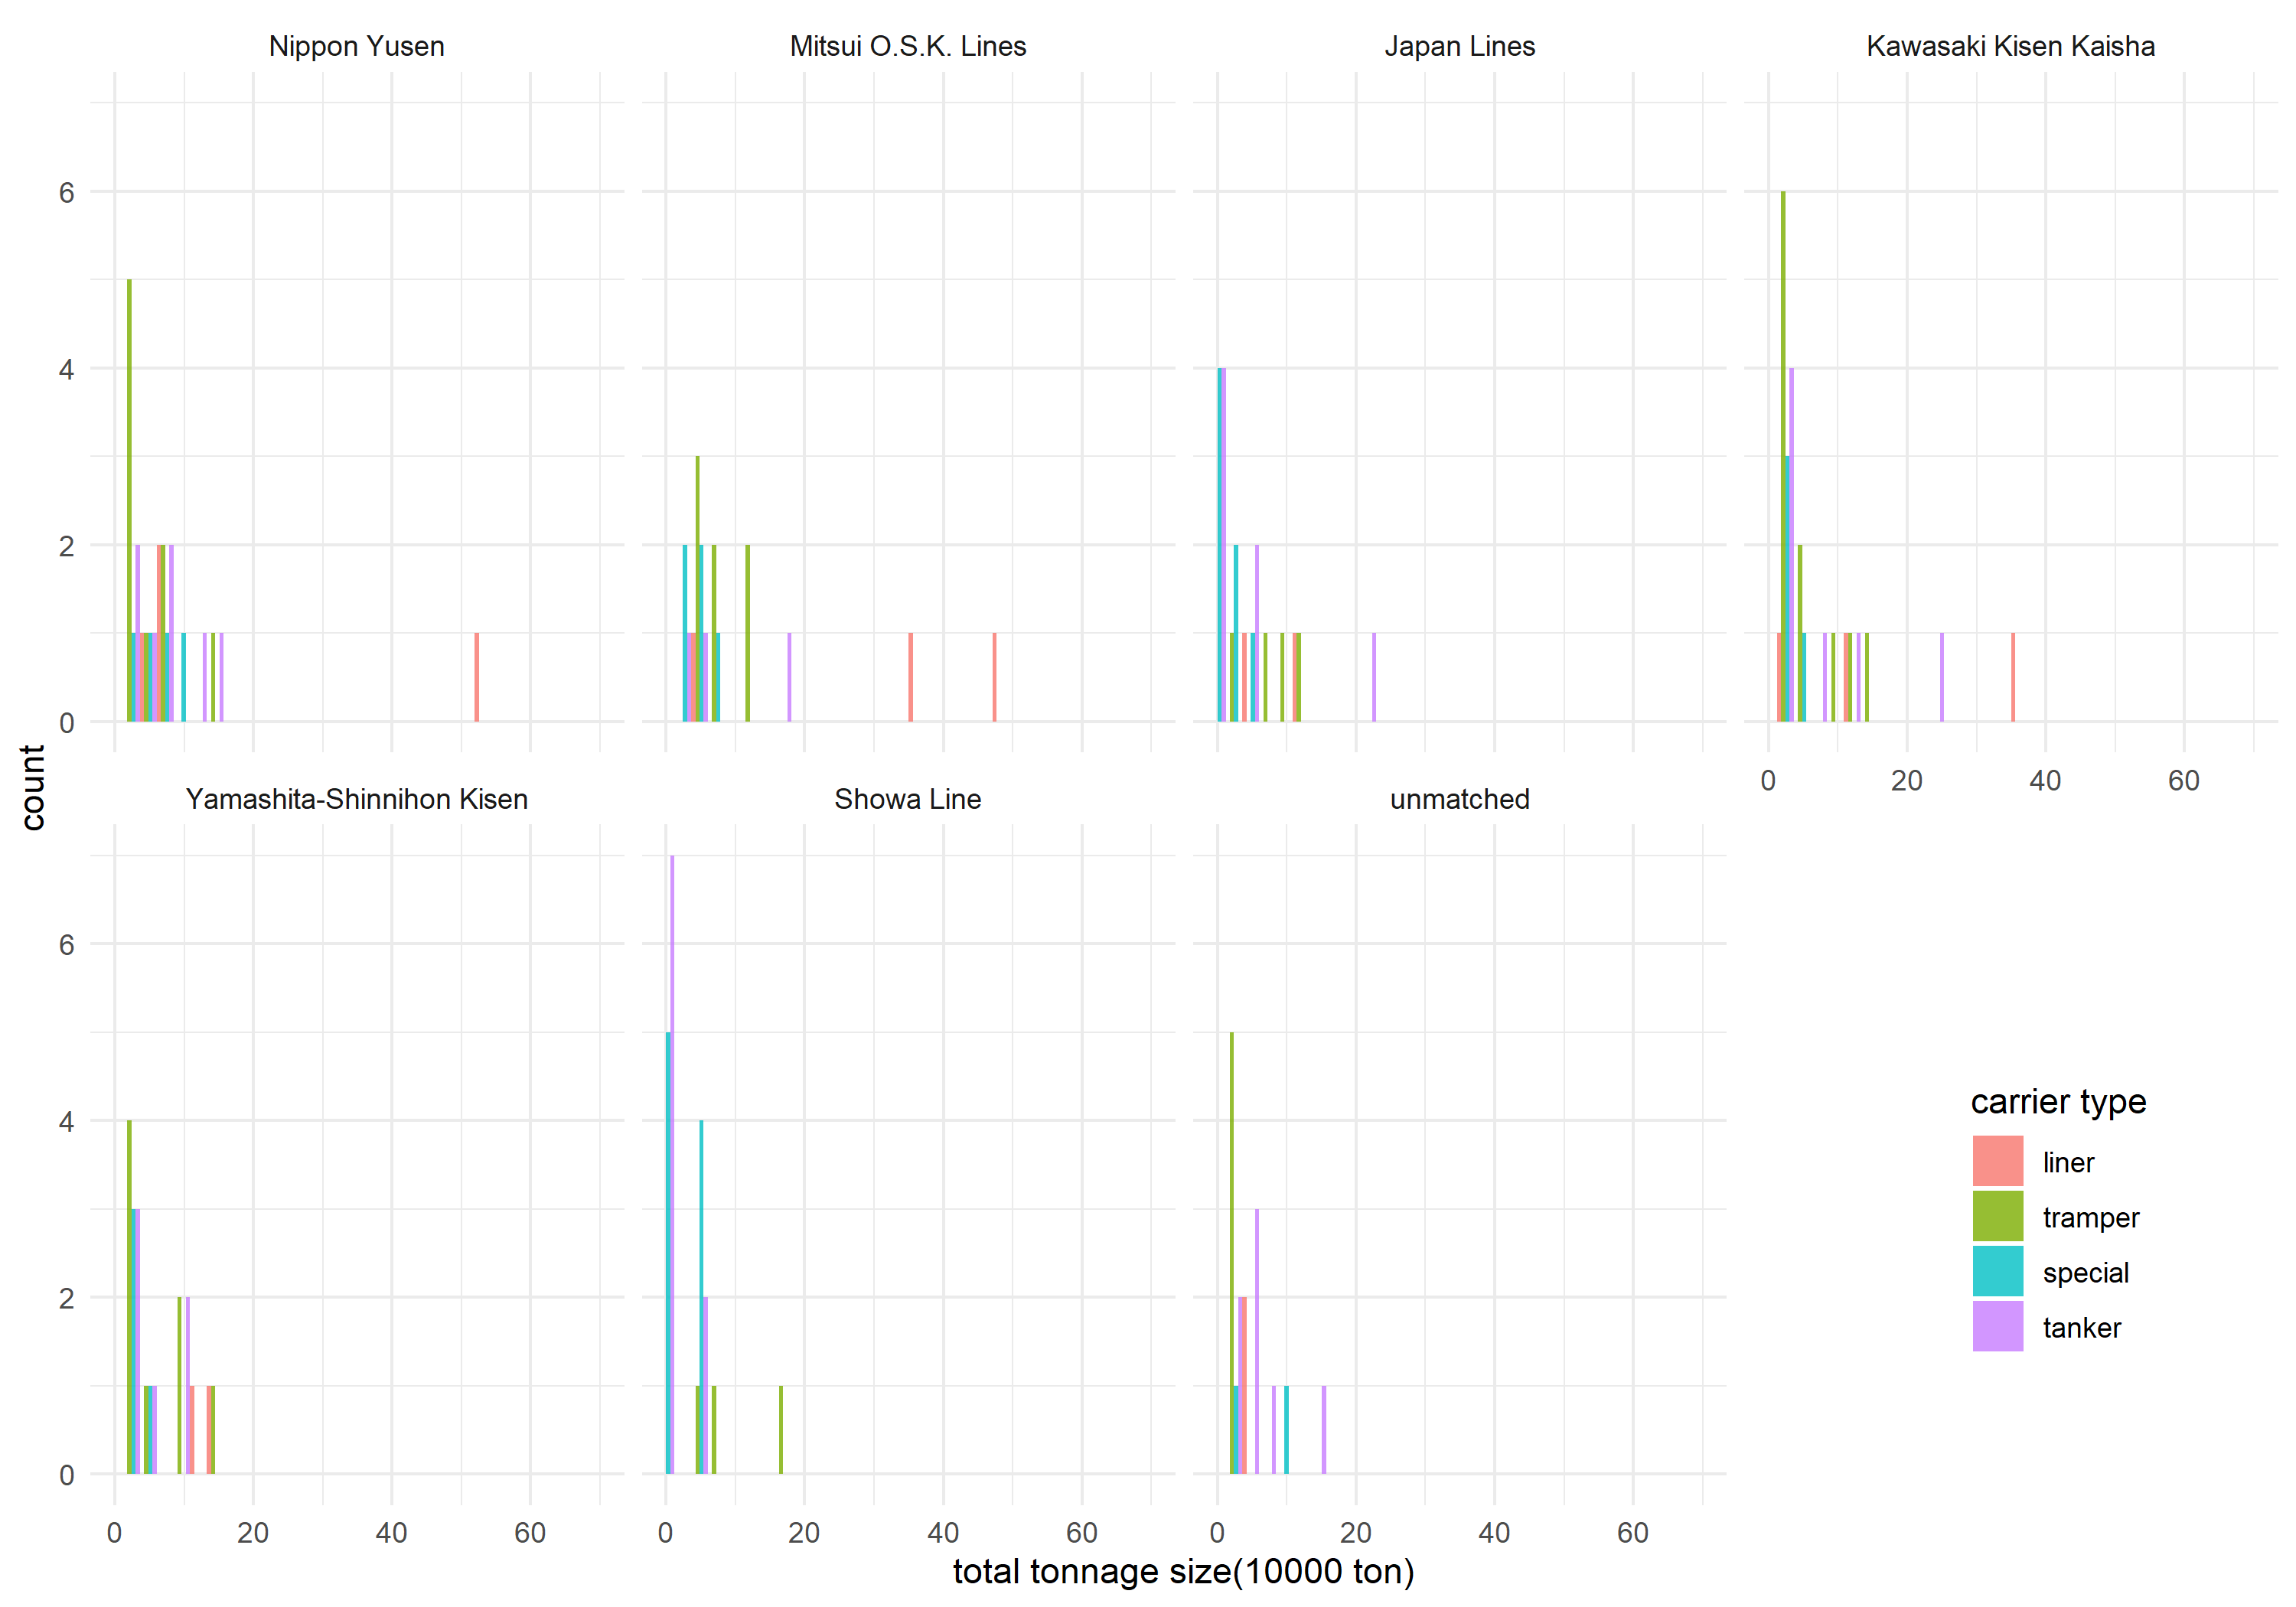
\includegraphics[height = 0.37\textheight]{../figuretable/carrier_dist_eachgroup.png}
\end{center}
\caption{\textbf{Distribution of tonnage size for each carrier type}. Observation unit: firm-level tonnage size for each carrier type of each group after mergers. }
\label{fg:carrier_dist_eachgroup}
\end{figure}

\hypertarget{figure-5-pie-charts}{%
\subsection{(Figure 5) Pie charts}\label{figure-5-pie-charts}}

\begin{figure}[!ht]
\begin{center}
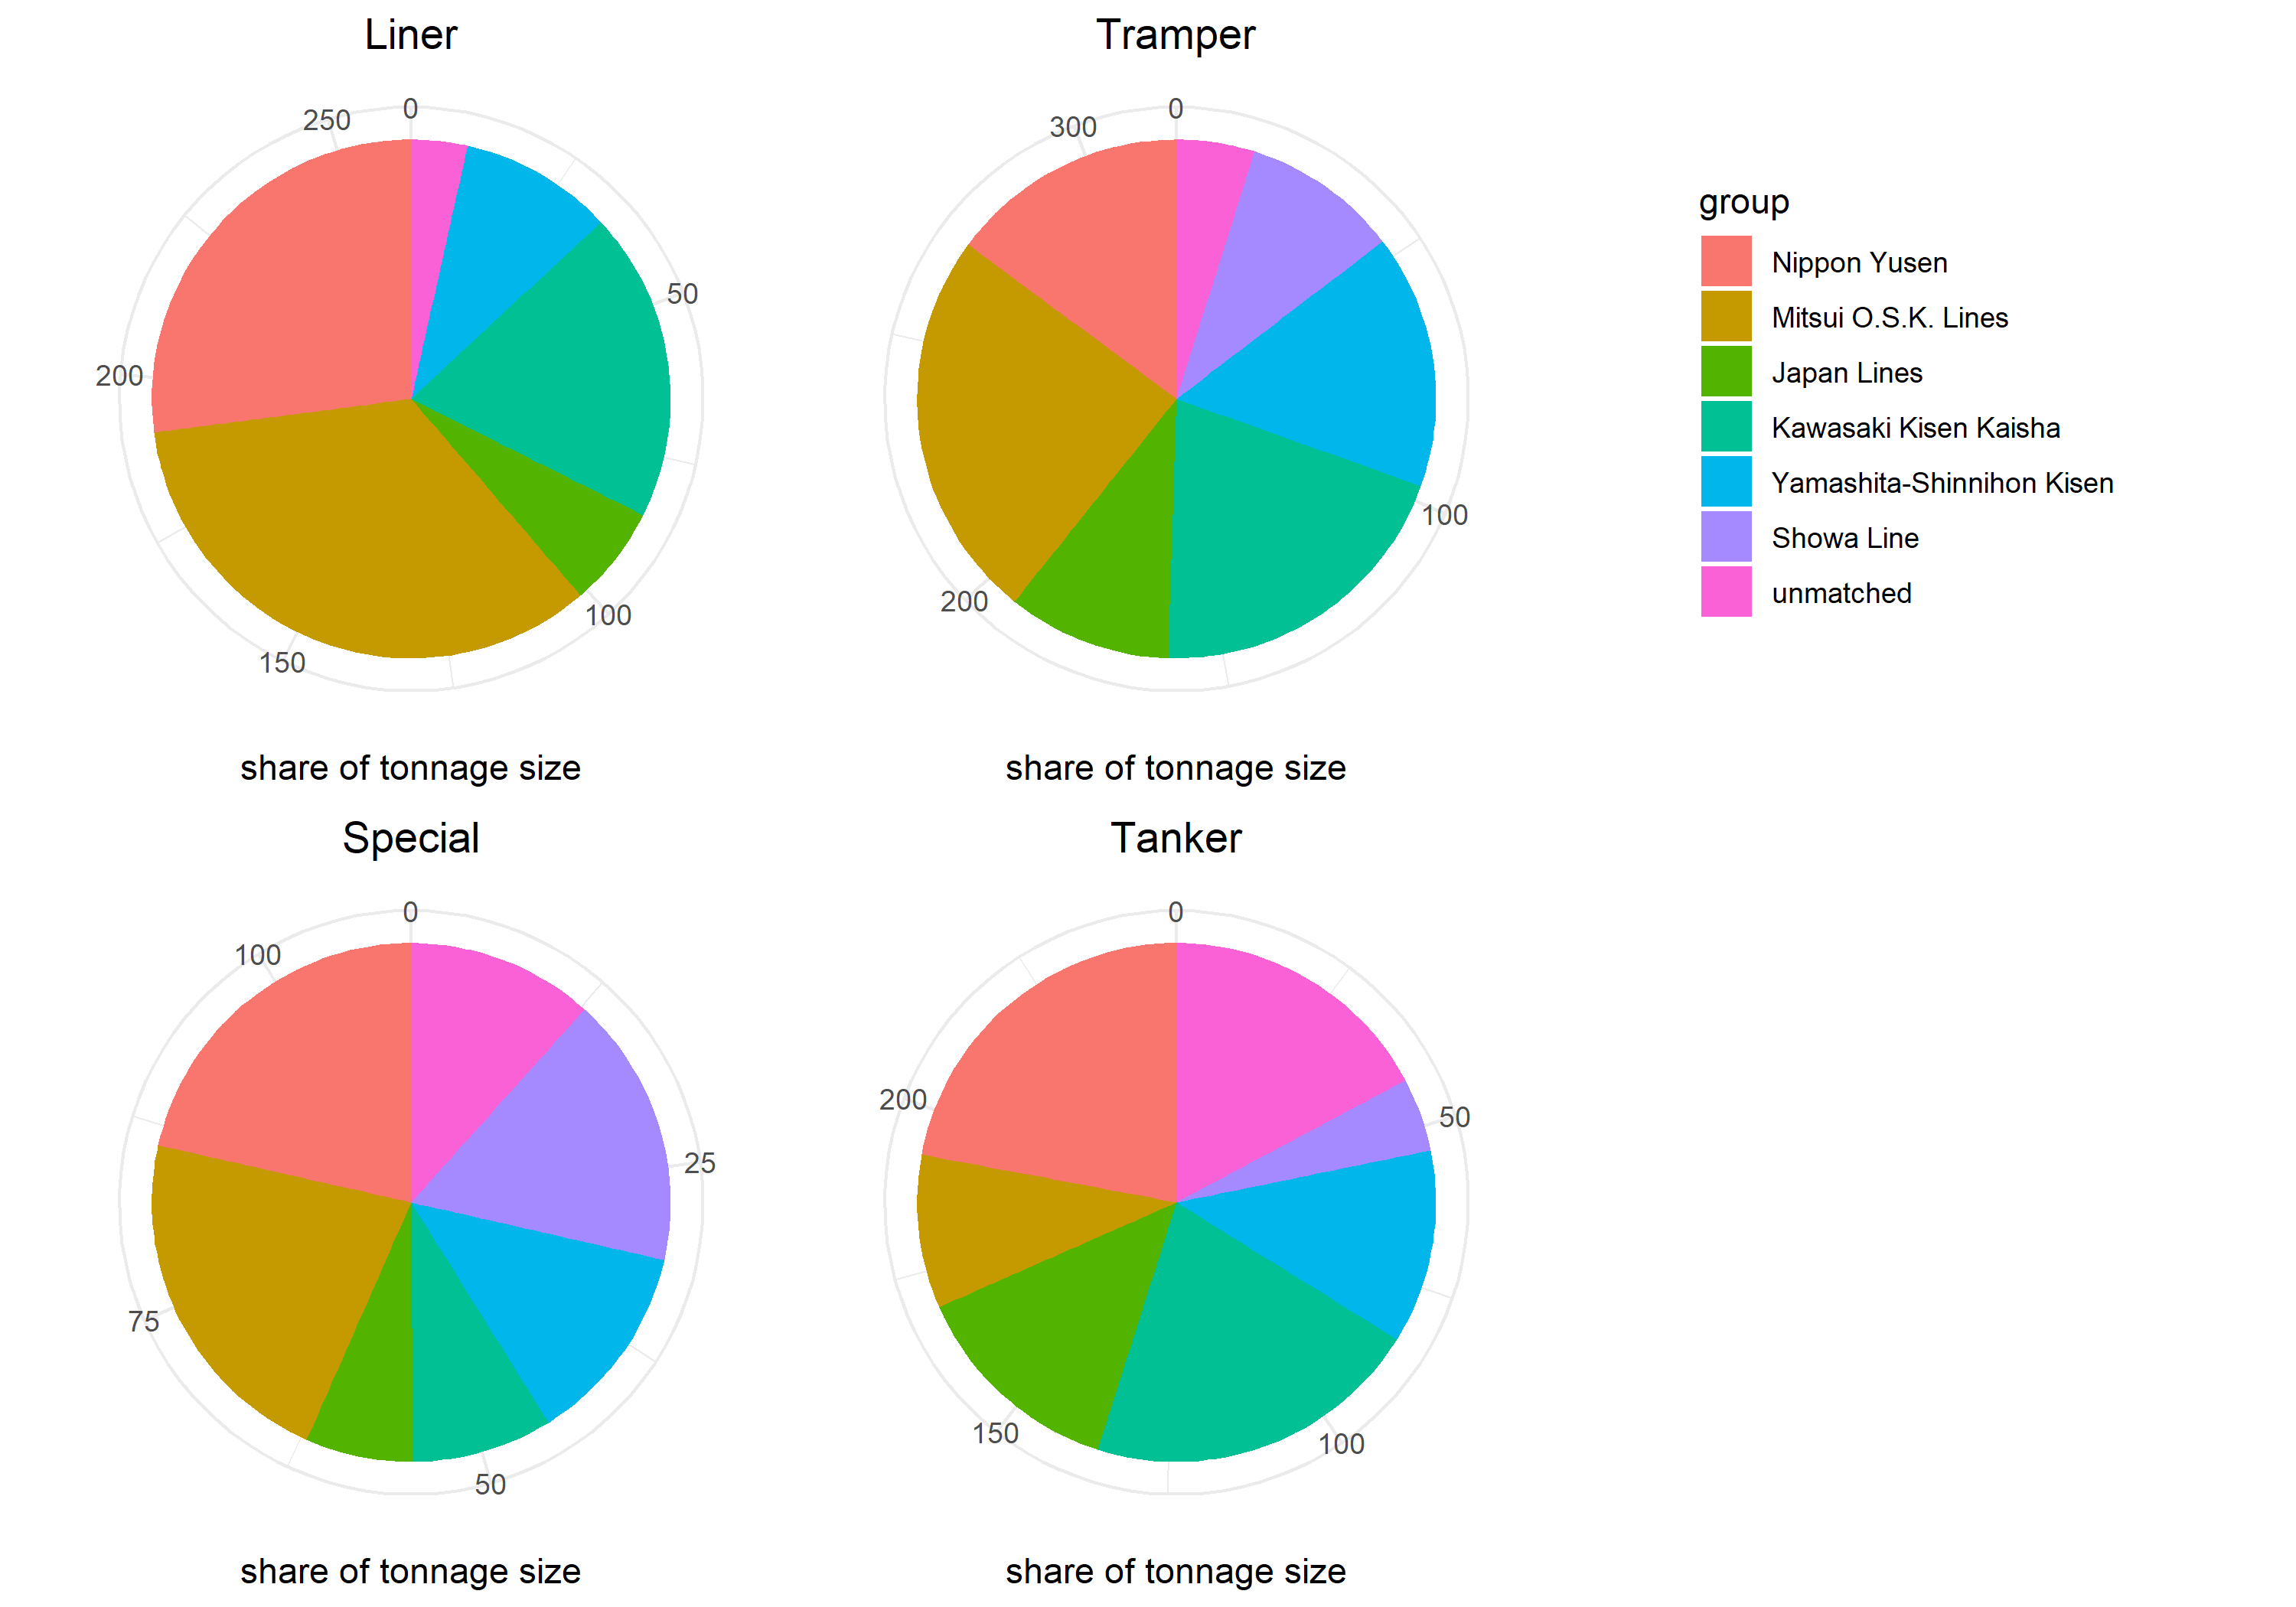
\includegraphics[height = 0.37\textheight]{../figuretable/carrier_share_eachgroup.png}
\end{center}
\caption{\textbf{Shares of each carrier type and each group}. Observation unit: group-level tonnage size for each carrier type after mergers. }
\label{fg:carrier_share_eachgroup}
\end{figure}

\hypertarget{descriptive-summary}{%
\section{Descriptive summary}\label{descriptive-summary}}

\hypertarget{table-3-summary-statistics-for-independent-variables.}{%
\subsection{(Table 3) Summary statistics for independent
variables.}\label{table-3-summary-statistics-for-independent-variables.}}

\begin{table}[!ht]
\scriptsize
\caption{\textbf{Summary statistics for independent variables}. \textit{Source} : \cite{listgaikou} and \cite{nostalgic}.}
\label{tb:shipping_market_stats_table}
\begin{center}
%latex.default(file = table_name, title = "", booktabs = TRUE,     object = temp, col.just = rep("r", dim(temp)[2]), center = "none",     table.env = FALSE, cgroupTexCmd = "itshape", colnamesTexCmd = "itshape",     collabel.just = rep("r", dim(temp)[2]), rgroupTexCmd = "itshape",     n.rgroup = c(5, 5), rgroup = c("Size variables (million (D/W) tons)",         "Specialization variables (\\% share)"))%
\begin{tabular}{lrrrrrrrr}
\toprule
\multicolumn{1}{l}{\itshape }&\multicolumn{1}{r}{\itshape N}&\multicolumn{1}{r}{\itshape mean}&\multicolumn{1}{r}{\itshape sd}&\multicolumn{1}{r}{\itshape min}&\multicolumn{1}{r}{\itshape q25}&\multicolumn{1}{r}{\itshape q50}&\multicolumn{1}{r}{\itshape q75}&\multicolumn{1}{r}{\itshape max}\tabularnewline
\midrule
{\itshape Size variables (million (D/W) tons)}&&&&&&&&\tabularnewline
~~total tonnage size&$118$&0.110&0.207&0.000&0.011&0.026&0.091&1.023\tabularnewline
~~total tonnage size of liner&$118$&0.031&0.112&0.000&0.000&0.000&0.000&0.721\tabularnewline
~~total tonnage size of special&$118$&0.015&0.033&0.000&0.000&0.000&0.008&0.177\tabularnewline
~~total tonnage size of tanker&$118$&0.030&0.071&0.000&0.000&0.000&0.024&0.417\tabularnewline
~~total tonnage size of tramper&$118$&0.035&0.055&0.000&0.002&0.013&0.034&0.246\tabularnewline
\midrule
{\itshape Specialization variables (\% share)}&&&&&&&&\tabularnewline
~~share of liner&$118$&0.104&0.235&0.000&0.000&0.000&0.000&1.000\tabularnewline
~~share of special&$118$&0.117&0.244&0.000&0.000&0.000&0.088&1.000\tabularnewline
~~share of tanker&$118$&0.192&0.351&0.000&0.000&0.000&0.208&1.000\tabularnewline
~~share of tramper&$118$&0.587&0.417&0.000&0.135&0.705&1.000&1.000\tabularnewline
~~HHI based on carrier types&$118$&0.815&0.241&0.258&0.584&1.000&1.000&1.000\tabularnewline
\bottomrule
\end{tabular}

\end{center}
\end{table}

\hypertarget{table-4-regression}{%
\subsection{(Table 4) Regression}\label{table-4-regression}}

\begin{table}[!ht]
\scriptsize
\caption{\textbf{Preliminary regression results for predicting matchings}. Observation unit: a one-to-one matching pair. The sample size is determined by all possible matching pairs from 118 firms in my data set. }
\begin{center}

\begin{tabular}{@{\extracolsep{5pt}}lccccc} 
\\[-1.8ex]\hline 
\hline \\[-1.8ex] 
 & \multicolumn{5}{c}{\textit{Dependent variable:}} \\ 
\cline{2-6} 
\\[-1.8ex] & \multicolumn{5}{c}{1(match)} \\ 
\\[-1.8ex] & (1) & (2) & (3) & (4) & (5)\\ 
\hline \\[-1.8ex] 
 log(liner$_{b}$ *liner$_{t}$+1) & $-$0.002 &  & $-$0.013 & $-$0.029 & $-$0.003 \\ 
  & (0.006) &  & (0.009) & (0.010) & (0.001) \\ 
  & & & & & \\ 
 log(tramper$_{b}$ *tramper$_{t}$+1) & 0.005 &  & 0.004 & 0.018 & 0.002 \\ 
  & (0.002) &  & (0.005) & (0.006) & (0.001) \\ 
  & & & & & \\ 
 log(special$_{b}$ *special$_{t}$+1) & $-$0.009 &  & $-$0.002 & $-$0.017 & $-$0.002 \\ 
  & (0.004) &  & (0.006) & (0.006) & (0.001) \\ 
  & & & & & \\ 
 log(tanker$_{b}$ *tanker$_{t}$+1) & $-$0.003 &  & $-$0.017 & $-$0.026 & $-$0.003 \\ 
  & (0.004) &  & (0.007) & (0.007) & (0.001) \\ 
  & & & & & \\ 
 log(total$_{b}$ *total$_{t}$+1) & $-$0.021 &  & $-$0.010 & 0.049 & 0.006 \\ 
  & (0.013) &  & (0.017) & (0.018) & (0.002) \\ 
  & & & & & \\ 
 bank coverage similarity ratio &  & 1.598 & 2.052 & 0.649 & 0.088 \\ 
  &  & (0.525) & (0.575) & (0.617) & (0.076) \\ 
  & & & & & \\ 
 log(HHI$_{b}$ *HHI$_{t}$+1) &  & 0.525 & 0.372 & $-$0.123 & $-$0.019 \\ 
  &  & (0.148) & (0.221) & (0.231) & (0.028) \\ 
  & & & & & \\ 
 log(share of liner$_{b}$ *share of liner$_{t}$+1) &  & 0.334 & 1.159 & 2.140 & 0.253 \\ 
  &  & (0.473) & (0.739) & (0.788) & (0.096) \\ 
  & & & & & \\ 
 log(share of special$_{b}$ *share of special$_{t}$+1) &  & $-$0.996 & $-$0.990 & $-$0.529 & $-$0.041 \\ 
  &  & (0.519) & (0.667) & (0.694) & (0.072) \\ 
  & & & & & \\ 
 log(share of tramper$_{b}$ *share of tramper$_{t}$+1) &  & 0.308 & 0.165 & $-$0.558 & $-$0.058 \\ 
  &  & (0.091) & (0.188) & (0.200) & (0.024) \\ 
  & & & & & \\ 
 log(share of tanker$_{b}$ *share of tanker$_{t}$+1) &  & 0.257 & 0.992 & 1.311 & 0.158 \\ 
  &  & (0.210) & (0.335) & (0.354) & (0.043) \\ 
  & & & & & \\ 
 same type &  &  &  & 1.600 & 0.229 \\ 
  &  &  &  & (0.052) & (0.007) \\ 
  & & & & & \\ 
 Intercept & $-$1.271 & $-$2.041 & $-$1.748 & $-$3.312 & $-$0.033 \\ 
  & (0.260) & (0.083) & (0.395) & (0.425) & (0.051) \\ 
  & & & & & \\ 
\hline \\[-1.8ex] 
Model & Logit & Logit & Logit & Logit & OLS \\ 
Observations & 13,806 & 13,806 & 13,806 & 13,806 & 13,806 \\ 
Akaike Inf. Crit. & 12,056.510 & 12,037.120 & 12,034.740 & 11,053.080 & 10,230.180 \\ 
\hline 
\hline \\[-1.8ex] 
\end{tabular} 

\end{center}
\label{tb:regression_matching}
\end{table}

\hypertarget{table-2-summary-of-total-tonnage-size-for-each-group}{%
\subsection{(Table 2) Summary of total tonnage size for each
group}\label{table-2-summary-of-total-tonnage-size-for-each-group}}

\begin{table}[!ht]
\scriptsize
\caption{\textbf{Summary of total tonnage size for each group}. \textit{Source} : \cite{listgaikou} and \cite{nostalgic}.}
\begin{center}
%latex.default(file = table_name, title = "", booktabs = TRUE,     object = data_english_for_reg_table, col.just = c("l", "r",         "r", "r"), center = "none", table.env = FALSE, rgroupTexCmd = "itshape",     n.rgroup = c(3, 3, 3, 3, 3, 3, 1, 1), rgroup = c("Nippon Yusen",         "Mitsui OSK Line", "Japan Line", "Kawasaki Kisen Kaisha",         "Yamashita Shinnihon Kisen", "Showa Line", "Unmatched",         "Total"))%
\begin{tabular}{llrrr}
\toprule
\multicolumn{1}{l}{}&\multicolumn{1}{c}{firm type}&\multicolumn{1}{c}{total tonnage}&\multicolumn{1}{c}{number of firms}&\multicolumn{1}{c}{total tonnage in a group}\tabularnewline
\midrule
{\itshape Nippon Yusen}&&&&\tabularnewline
~~1&(1) main&1509795&2&2577274\tabularnewline
~~2&(2) affiliate&841568&7&\tabularnewline
~~3&(3) wholly controlled&225911&7&\tabularnewline
\midrule
{\itshape Mitsui OSK Line}&&&&\tabularnewline
~~4&(1) main&1924859&2&2879216\tabularnewline
~~5&(2) affiliate&400530&5&\tabularnewline
~~6&(3) wholly controlled&553827&20&\tabularnewline
\midrule
{\itshape Japan Line}&&&&\tabularnewline
~~7&(1) main&1122694&2&1328069\tabularnewline
~~8&(2) affiliate&125738&1&\tabularnewline
~~9&(3) wholly controlled&79637&4&\tabularnewline
\midrule
{\itshape Kawasaki Kisen Kaisha}&&&&\tabularnewline
~~10&(1) main&1658650&2&2338502\tabularnewline
~~11&(2) affiliate&391170&9&\tabularnewline
~~12&(3) wholly controlled&288682&7&\tabularnewline
\midrule
{\itshape Yamashita Shinnihon Kisen}&&&&\tabularnewline
~~13&(1) main&899033&2&1671590\tabularnewline
~~14&(2) affiliate&601616&5&\tabularnewline
~~15&(3) wholly controlled&170941&10&\tabularnewline
\midrule
{\itshape Showa Line}&&&&\tabularnewline
~~16&(1) main&549095&2&1041063\tabularnewline
~~17&(2) affiliate&464830&3&\tabularnewline
~~18&(3) wholly controlled&27138&4&\tabularnewline
\midrule
{\itshape Unmatched}&&&&\tabularnewline
~~19&unmatched&1131211&24&1131211\tabularnewline
\midrule
{\itshape Total}&&&&\tabularnewline
~~20&&12966925&118&12966925\tabularnewline
\bottomrule
\end{tabular}

\end{center}
\label{tb:total_tonnage_size_group_table}
\end{table}

\hypertarget{export-dataset-for-maximum-rank-estimator}{%
\section{Export dataset for maximum rank
estimator}\label{export-dataset-for-maximum-rank-estimator}}

\hypertarget{sankey-diagram-based-on-estimated-parameters}{%
\section{Sankey diagram based on estimated
parameters}\label{sankey-diagram-based-on-estimated-parameters}}

\hypertarget{figure-9-merger-simulation-across-different-subsidy-threshold-and-amount.}{%
\subsection{(Figure 9) Merger simulation across different subsidy
threshold and
amount.}\label{figure-9-merger-simulation-across-different-subsidy-threshold-and-amount.}}

Sankey diagrams need to be exported from a clipboard. For the draft, I
added information of x-axis (subsidy threshold and amount) manually to
the figures generated here. The data input of simulated merger
configurations is computed on ship\_merger\_counterfactual.jl.

\end{document}
